\documentclass[10pt,a4paper]{article} % tamaño de letra y tipo de papel
\usepackage[utf8]{inputenc}
\usepackage[spanish]{babel} % paquete para que reconozca ñ y tildes
\usepackage{amsmath}
\usepackage{upgreek} 
\usepackage{amsfonts}
\usepackage{amssymb}
\usepackage{graphicx} % paquete para incluir imagenes
\graphicspath{ {imagenes/}}
\usepackage[margin=1in,bottom=1in]{geometry}
\usepackage{hyperref} % paquete para tener marcadores en el pdf
\usepackage{tikz}
\usetikzlibrary{babel}
\usepackage[siunitx, RPvoltages]{circuitikz}
\usetikzlibrary{bending,arrows.meta,positioning,calc,positioning}
\usepackage{pgfplots}\pgfplotsset{compat=1.13}
\usepackage{float}
\usepackage[T1]{fontenc}
\usepackage[numbered,framed]{matlab-prettifier}
\pgfplotsset{width=12cm,legend style={at={(0.11,0.75)},anchor=south},select coords between index/.style 2 args={
		x filter/.code={
			\ifnum\coordindex<#1\def\pgfmathresult{}\fi
			\ifnum\coordindex>#2\def\pgfmathresult{}\fi
		}
}}
\author{Ulloa Daniel & Rodriguez Victoria}
\begin{document}

\begin{titlepage}
	\hbox{
		\hspace*{0.15\textwidth} % Espacio desde el margen izquierdo
		\rule{1pt}{\textheight} % Linea decorativa
		\hspace*{0.05\textwidth} % Espacio entre la linea y el texto
		\parbox[b]{0.75\textwidth}{ % Caja que restringe el espacio que puede ocupar el texto
			{\noindent\Huge\bfseries Informe de Laboratorio } % Titulo
			\\ 
			[2\baselineskip] 
			{\large \textbf{Tema:} Medición de respuestas
				temporal y frecuencial} % Tema
			\\[4\baselineskip]
            {\large \textbf{Cátedra:} Teoría de Circuitos \textsc{II}} % Catedra
            \\[1\baselineskip]
            {\large \textbf{Año:} 2019} % Año
			\\[1\baselineskip]
            {\large \textit{\textbf{Docentes:} % Docentes
                \textnormal{Ing. Costa}, Nicolás. 
                \textnormal{Aux. Consiglio}, Dante}
            }
			\\[1\baselineskip]
            {\large \textit{\textbf{Alumnos:} % Alumnos
                \textnormal{Rodriguez}, Ana Victoria. 
                \textnormal{Ulloa}, Daniel Alejandro}
            }
            \\[6\baselineskip]
            {\large \textbf{Fecha de Entrega:} 08/10/2019}
			\par %Para que el logo aparezca al pie
			\vspace{0.35\textheight} % Ubicacion de la caja desde el margen superior
            \center{
\includegraphics[width=250px]{logo2.png}}
            \\[1\baselineskip]
	}}
\end{titlepage}
\tableofcontents
\newpage

\section{Objetivos}
\begin{itemize}
    \item Modelar e interpretar el circuito
    \item Realizar los gráficos de Bode correspondiente al circuito
    \item Obtener la función de transferencia a partir de la respuesta al escalón
\end{itemize}

\section{Modelado Matemático}
 %inserte aquí el circuito que seguro hará Daniel, porque es una perra :3
\begin{itemize}
	\item Los amplificadores operacionales son ideales
	\item La salida del sistema es la tensión a la salida del segundo amplificador operacional
\end{itemize}
Para la primera ecuación se analizó el nodo $V_2$, en donde se tiene que:
\begin{align}
\frac{V_2-V_1}{R_1}+V_2sC_1=0
\end{align}
Se define la ecuación de la tensión de salida como
\begin{align}
\frac{V_o-V_2}{R_2}+V_osC_1=0
\end{align}
Con estas dos ecuaciones es posible obtener la función de transferencia del sistema
\begin{align}
H(s)=\frac{1}{s^2(C1C2R1R2)+s(C1R1+C2R2)+1}
\end{align}
 Se realizo el correspondiente diagrama de bode, mediante Mathematica, obteniendo lo siguiente
\begin{figure}[H]
\begin{center}
	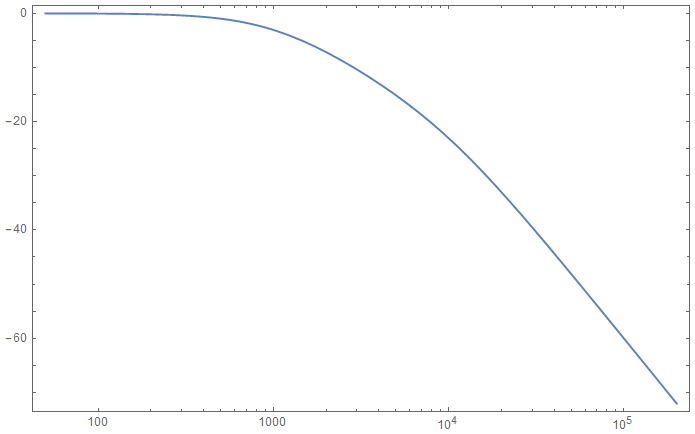
\includegraphics[scale=0.5]{bode1}
	\caption{Amplitud}
\end{center}
\end{figure}
\begin{figure}[H]
	\begin{center}
		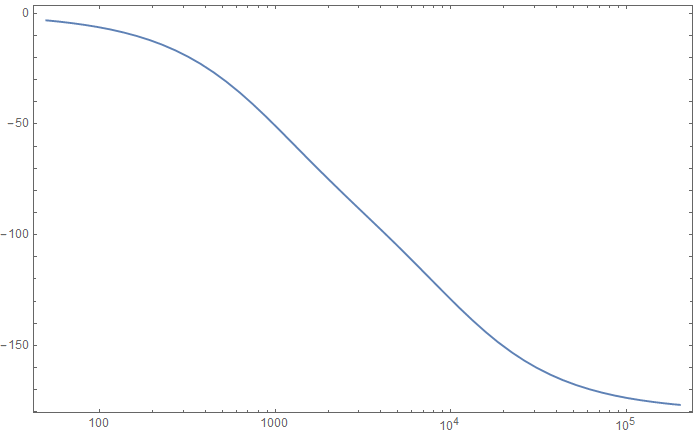
\includegraphics[scale=0.5]{bode2}
		\caption{Fase}
	\end{center}
\end{figure}
Se concluye a partir de la función de transferencia y el diagrama de bode que el circuito presentado conforma un sistema de segundo orden y que el mismo es un filtro pasabajos.

Por último se obtuvo otro diagrama de bode esta vez simulando el sistema mediante el programa Lt Spice. 
\begin{figure}[H]
	\begin{center}
		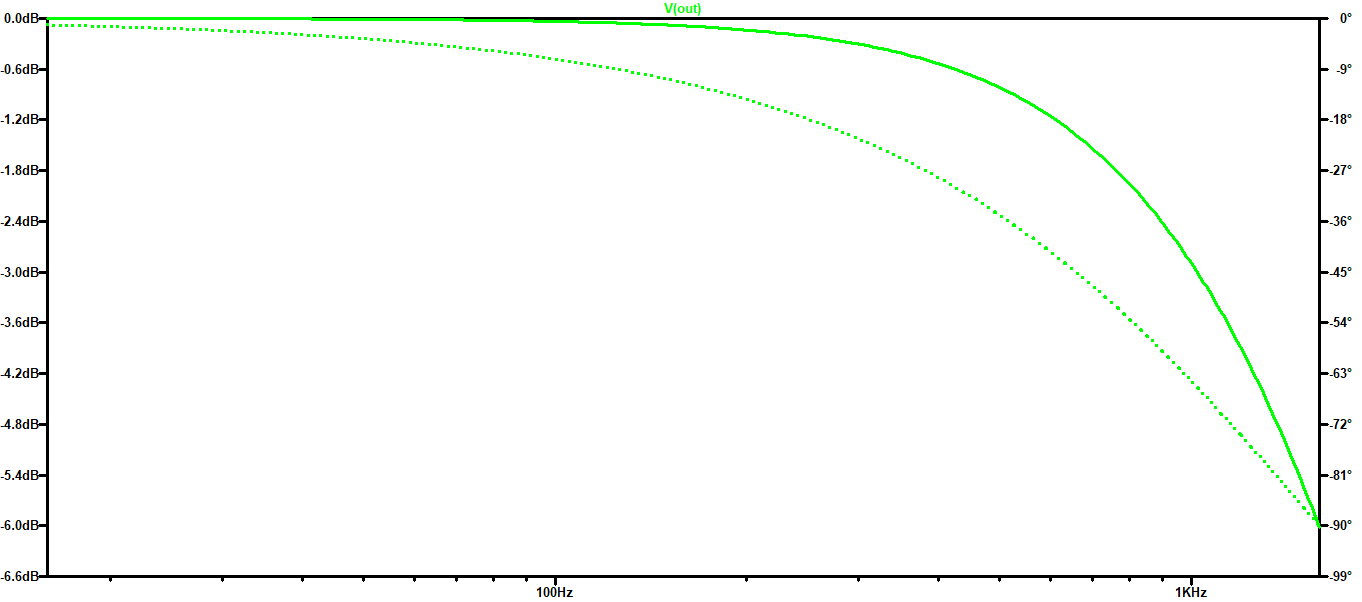
\includegraphics[scale=0.4]{bode3}
		\caption{Amplitud(Línea continua) y Fase(Linea puntuada)}
	\end{center}
\end{figure}
\section{asdasdasda}

Se implementó el sistema en un protoboard con un generador de funciones y un osciloscopio digital para visualizar la salida y la entrada. Para poder realizar un barrido de frecuencia se vario la frecuencia de la entrada y se tomo los datos de la tensión de la entrada y salida. 
Para cada frecuencia se guardo un archivo .csv en un pendrive y se realizó un script en matlab para obtener un diagrama de bode con los datos medidos.

\begin{figure}[H]
	\begin{center}
		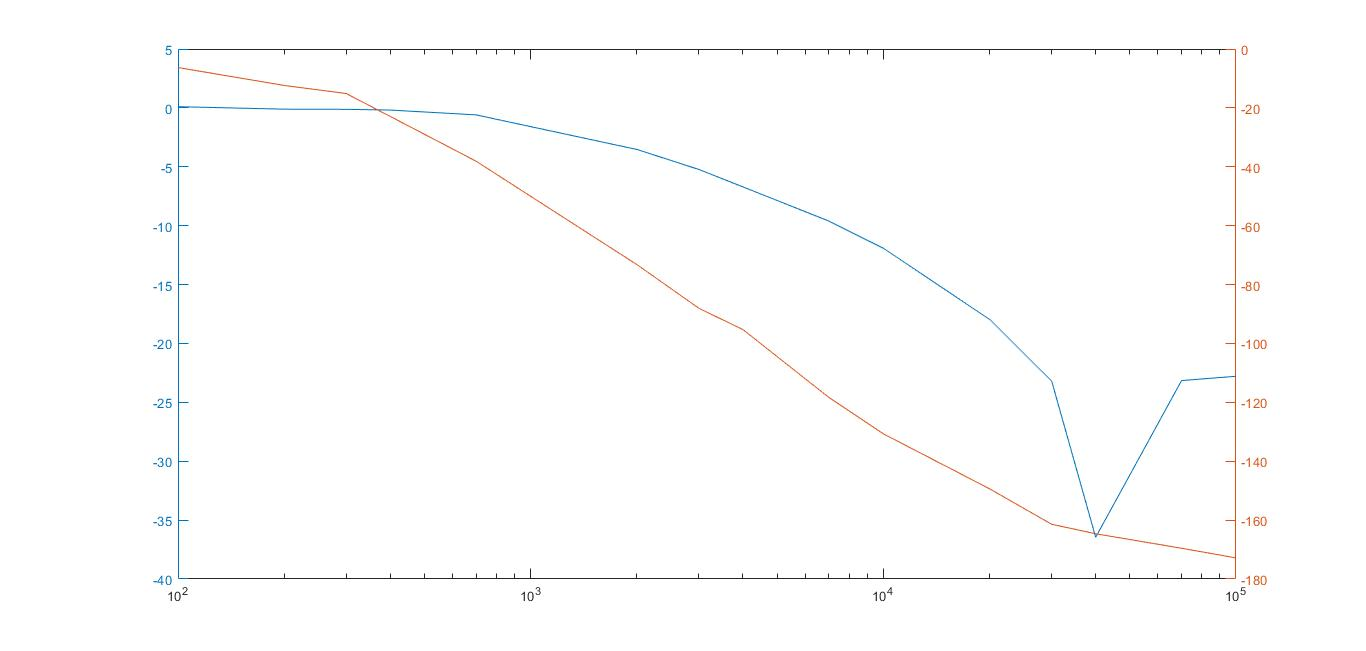
\includegraphics[scale=0.4]{bode4}
		\caption{Amplitud(Línea azul) y Fase(Linea Rojo)}
	\end{center}
\end{figure}


\section{Conclusión}




\end{document} 
